% !TEX TS-program = pdflatex
% !TEX encoding = UTF-8 Unicode
\documentclass[11pt]{article} % use larger type; default would be 10pt

\usepackage[utf8]{inputenc} % set input encoding (not needed with XeLaTeX)
\usepackage{multirow}
\usepackage{footnote}

%%% Examples of Article customizations
% These packages are optional, depending whether you want the features they provide.
% See the LaTeX Companion or other references for full information.

%%% PAGE DIMENSIONS
\usepackage{geometry} % to change the page dimensions
\geometry{a4paper}

\usepackage{graphicx} % support the \includegraphics command and options
\graphicspath{ {./images/} }


%%% PACKAGES
\usepackage{booktabs} % for much better looking tables
\usepackage{array} % for better arrays (eg matrices) in maths
\usepackage{paralist} % very flexible & customisable lists (eg. enumerate/itemize, etc.)
\usepackage{verbatim} % adds environment for commenting out blocks of text & for better verbatim
\usepackage{subfig} % make it possible to include more than one captioned figure/table in a single float

%%% HEADERS & FOOTERS
\usepackage{fancyhdr}
\pagestyle{fancy}
\renewcommand{\headrulewidth}{0pt} % customise the layout...
\lhead{}\chead{}\rhead{}
\lfoot{}\cfoot{\thepage}\rfoot{}

%%% SECTION TITLE APPEARANCE
\usepackage{sectsty}
\allsectionsfont{\sffamily\mdseries\upshape} % (See the fntguide.pdf for font help)

%%% ToC (table of contents) APPEARANCE
\usepackage[nottoc,notlof,notlot]{tocbibind} % Put the bibliography in the ToC
\usepackage[titles,subfigure]{tocloft} % Alter the style of the Table of Contents
\renewcommand{\cftsecfont}{\rmfamily\mdseries\upshape}
\renewcommand{\cftsecpagefont}{\rmfamily\mdseries\upshape} % No bold!

%%% END Article customizations

%%% The "real" document content comes below...



\begin{document}
\title{\vspace{-2cm}BloomFilter - Diskrete Stochastik 2020}
\author{Sebastian Fernandez}
\date{}
\maketitle

\section{Idee, Vor- und Nachteile}
Ein Bloomfilter ist eine Speichereffiziente auf Wahrscheinlilchkeiten basierende Datenstruktur. Die Elemente in der Menge können nicht ausgegeben werden, sondern es kann nur geprüft werden, ob ein Element in der Menge enthalten ist oder nicht. Dabei können False-Positiv Überprüfungen vorkommen, nicht jedoch False-Negativ. Elemente können also bei der Überprüfung "möglicherweise" in der Menge enthalten oder "definitiv nicht" in der Menge sein. Elemente können nur hinzugefügt werden, nicht jedoch von der Menge entfernt werden.
	\subsection {Vorteile}
		\begin{itemize}
    			\item Konzept des BloomFilters ist leicht zu verstehen und gut dokumentiert.
 			\item Laufzeitkomplexität, Elemente können mit O(k) hinzugeügt oder auf dessen Existenz überprüft werden. Das heisst, dass Elemente für beide Operationen nur auf die zuvor definierte Anzahl k Hashfunktionen angewandt werden muss. Die Laufzeit wird durch das hinzufügen von Elementen nicht erhöht, mit dem Preis einer erhöhter Wahrscheinlichkeit für False-Positive Überprüfungen.
 			\item Sofern die Anzahl Elemente abgeschätzt werden kann und eine gewisse Fehlertolleranz akzeptiert wird, besteht ein Vorteil in seinem geringen Speicherverbauch. Ist die Anzahl Elemente jedoch nicht im geringsten abzuschätzen, wird entweder ein zu kleine Datenstruktur vordefiniert, welches zu hohen False-Positiv Werten führt, oder aber es wird unnötig Speicherplatz reserviert.
		\end{itemize}
	\subsection {Nachteile}
		\begin{itemize}
			\item Das entfernen von Elementen ist nicht möglich, da ein einzelner Bit-Wert von mehreren Elementen genutzt werden kann. Der Bit-Wert kann also nicht einfach auf 0 gesetzt werden, weil nicht bestimmt werden kann, inwiefern andere Elemente das Bit verwenden. Bei einer zu hohen False-Positiv Rate muss der Bloomfilter von Grundauf neu aufgebaut werden.
			\item Auslesen der Elemente ist nicht möglich, nur die wahrscheinliche Überprüfung ob ein gewisses Element vorhanden ist. Wenn das Element jedoch nicht vorhanden ist, dann ist die Überprüfung korrekt und der erwartete Wert "false" wird zurückgegeben.
			\item Eingeschränkte Verwendungsmöglichkeit, da die Anzahl hinzugefügter Elemente bekannt oder abschätzbar sein muss. Wenn die Grösse nicht bekannt ist, kann die Verwendung des Bloomfilters zu inakzeptablen Resultaten führen.
		\end{itemize}

\section{Praxisbeispiel - BloomFilter}

Mittels Bloomfilter kann mit Sicherheit festgestellt werden, ob ein Element nicht in einer Menge vorhanden ist. Diese Eigenschaft kann bei teuren oder häufig durchgeführten Datenbankabfragen angewendet werden. Angenommen wir haben eine spezifisches Query auf einen Datenbankserver, welche 10'000-Mal/Sekunde überprüft, ob ein Benutzer existiert oder nicht. Ein Bloomfilter kann vor dieser Datenbankabfrage eingeführt werden, um zu ermitteln, ob der angefrage Nutzer überhaupt existiert. Wenn der Benutzer gar nicht erst vorhanden ist, muss keine teure Datenbankverbindung (TCP, 3-Way Handshake) aufgebaut werden, sowie auch die Abfrage nicht ausgeführt werden. Wenn der Benutzer existiert, man sich jedoch nicht ganz sicher ist, kann die Abfrage an den Datenbankserver immernoch durchgeführt werden. Der grosse Vorteil besteht darin, dass die Anzahl der Abfragen auf einen Datenbankserver minimiert werden kann.

\section{Tests}
Insgesamt wurden 4 dokumentierte Tests durchgeführt. Die 4 Tests wurden in zwei Gruppen, nach Grösse hinzugefügter Wörter, aufgeteilt. In der ersten Gruppe wurde jedes dritte Wort hinzugefügt. Mit den Restlichen Wörtern wurde die FP- Wahrscheinlichkeit überprüft und berechnet. 
Die zweite Gruppe enthält jedes zweite Wort aus der Wörterliste. Mit der anderen hälfte wurde die FP-Wahrscheinlichkeit überprüft und berechnet. Für jedes Element einer Gruppe wurden unterschiedliche FP Erwartungswerte gesetzt. Die untenstehende Tabelle zeigt die Resultate auf.

\begin{center}
\begin{tabular}{ |c|c|c|c|c|c| } 
\hline
Erwartet FP \footnotemark & Erreicht FP & Hinzugefügt & Überprüft & HashFunc \footnotemark & Arraygrösse \footnotemark \\
\hline
0.001 & ~0.00217 & 1/3 = 19'370 & 2/3 = 38'740 & 10 & 278494\\ 
0.01 & ~0.02070 & 1/3 = 19'370 & 2/3 = 38'740 &  7 & 185663 \\ 
0.001 & ~0.00110 & 1/2 = 29'055 & 1/2 & 10 & 417741\\ 
0.01 & ~0.01098 & 1/2 = 29'055 & 1/2 &  7 & 278494 \\ 
\hline
\end{tabular}


\end{center}

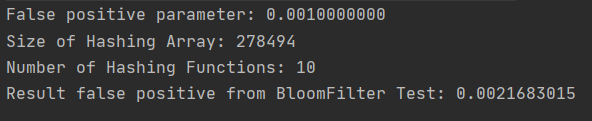
\includegraphics[width=12cm, height=2.5cm]{results_0_001FP}

\footnotetext[1]{False-Positiv Wahrscheinlichkeit (möglicherweise in der Menge enthalten)}
\footnotetext[2]{Anzahl der verwendeten Hash Funktionen}
\footnotetext[3]{Anzahl dem BloomFilter hinzugefügter Elemente }
\end{document}
